\documentclass[xcolor=dvipsnames]{beamer}
\usepackage{amsfonts, epsfig, xspace, relsize}
\usepackage{algorithm,algorithmic}
\usepackage{graphicx}
 \DeclareGraphicsExtensions{.pdf,.png,.jpg,.jpeg,.mps}
\renewcommand{\figurename}{圖}
\renewcommand{\tablename}{表}
\usepackage{pstricks,pst-node}
\usepackage{multimedia}
\usepackage{enumerate}
\usepackage[normal,tight,center]{subfigure}
\setlength{\subfigcapskip}{-.5em}
\usepackage{beamerthemesplit}
\usepackage{mathtools}
\usepackage{xcolor}
\usepackage{fancyvrb}
\usepackage{framed,color}
\definecolor{shadecolor}{rgb}{0.8,1,0.5}
\usepackage{amsmath}% http://ctan.org/pkg/amsmath
\usepackage[retainorgcmds]{IEEEtrantools}% http://ctan.org/pkg/ieeetran
\newcommand{\non}{\IEEEnonumber*}
\newcommand\independent{\protect\mathpalette{\protect\independenT}{\perp}}
\def\independenT#1#2{\mathrel{\rlap{$#1#2$}\mkern2mu{#1#2}}}

\setbeamertemplate{caption}[numbered]
\usepackage{fontspec}  %加這個就可以設定字體
\usepackage{xeCJK}       %讓中英文字體分開設置
%\setromanfont{LiHei Pro} % 儷黑Pro
\newCJKfontfamily{\K}{標楷體}
\newCJKfontfamily{\H}{微軟正黑體}
\setmonofont[Scale=0.8]{Courier New} % 等寬字型
\setmainfont{Times New Roman}
\setsansfont{Times New Roman}
\setCJKmainfont{王漢宗細圓體繁} %設定中文為系統上的字型,而英文不去更動,使用原TeX字型
\XeTeXlinebreaklocale "zh"             %這兩行一定要加,中文才能自動換行
\XeTeXlinebreakskip = 0pt plus 1pt     %這兩行一定要加,中文才能自動換行
%\usetheme{lankton-keynote}
\usetheme{Madrid}
\usecolortheme[named=BrickRed]{structure}
\author[蔡佳泓]{\K 蔡佳泓}

\title[Statistical Methods for Social Sciences]{Regression Analysis\\
\smallskip
{\small {Simple Linear Regression: Properties and Assumptions}}}
\date[5/16/2017]{2017年5月16日} %leave out for today's date to be insterted
\institute[ESC \& GIEAS]{\H 國立政治大學選舉研究中心暨東亞研究所}
\begin{document}
\maketitle
\begin{frame}{Outline}
\tableofcontents
\end{frame}

\section{OLS的統計特性}
\begin{frame}{\H 描述與推論}

\begin{itemize}
\item 到目前為止,我們用迴歸來描述資料,但是沒有用來推論。
\item $ E(Y|X) $,也就是條件平均值,也就是$Y$是$X$的函數,才是我們要估計的。
\[E[Y|X]=\beta_{0}+\beta_{1}X\]
\[\hat{E}[Y|X]=\hat{\beta_{0}}+\hat{\beta_{1}}\]
\[y_{i}=\hat{\beta_{0}}+\hat{\beta_{1}}+u_{i}\]
%\item 最小平方法迴歸有一連串的假設必須滿足
%\item 在這些假設成立的前提下,進行區間估計、假設檢定等等。
\end{itemize}
\end{frame}
\begin{frame}{散佈圖1}
\begin{figure}
\includegraphics[scale=.30]{"geompoint1.png"}
\caption{市區油耗與高速公路油耗的散佈圖}
\label{fig.1}
\end{figure}
\end{frame}
\begin{frame}{散佈圖2}
\begin{figure}
\includegraphics[scale=.30]{"geompoint2.png"}
\caption{去掉重複觀察值的散佈圖}
\label{fig.2}
\end{figure}
\end{frame}

\begin{frame}{散佈圖的觀察}
\begin{itemize}
\item 圖 \ref{fig.2} 顯示兩個變數之間有可能有正相關。當$X$軸的變數增加,$Y$的變數也增加。
\item 但是我們必須注意$X$軸的變數是否有不尋常的大或是小的值,影響與$Y$變數之間的關係。
\end{itemize}
\end{frame}
\begin{frame}{散佈圖加上迴歸線}
\begin{figure}
\includegraphics[scale=.4]{"weather.png"}
\caption{散佈圖加上迴歸線圖}
\label{fig.3}
\end{figure}
\end{frame}
\begin{frame}{散佈圖加上迴歸線圖的觀察}
\begin{itemize}
\item 圖\ref{fig.3}顯示,$X$與$Y$的關係有可能不強。
\end{itemize}
\end{frame}
\begin{frame}{折線圖}
\begin{figure}
\includegraphics[scale=.3]{"line1.png"}
\caption{折線圖}
\label{fig.4}
\end{figure}
\end{frame}
\begin{frame}{折線圖的觀察}
\begin{itemize}
\item 圖\ref{fig.4}顯示,每一個點代表給予不同來源的蛋氨酸的火雞的平均體重,因此每條線通過$E[Y|X]$,沒有
誤差。
\item 圖\ref{fig.4}也顯示,$X$與$Y$的關係可能不是線性。
\end{itemize}
\end{frame}
\begin{frame}{\H 母體模型}
\begin{itemize}
\item 預測模型可表示為 
\[ E[Y|X]=\beta_{0}+\beta_{1}X \]
\item 因為固定$X=x$時,$Y$有各種可能的值,也就是
\[Var[Y|X]=\sigma^2 \]
\item 因此母體模型可表示為: $y_{i}=E[Y|X]+u_{i}=\beta_{0}+\beta_{1}X+u_{i} $
\begin{itemize}
\item $Y$是依變數(outcome)
\item $X$是自變數(regressor)
\item $\beta_{0},\beta_{1}  $分別是截距以及斜率
\item $u$(或者$\epsilon$): 誤差項 (error terms, statistical errors),也是一個捕捉到所有會影響$Y$但不影響$X$的隨機變數。
\textcolor{red}{\K 誤差是$Y$與$E(Y|X)$之間的差距,也就是與真實的線性關係之間的差距,無法觀察。}
\end{itemize}
\item 估計模型則是:$Y=\hat{\beta_{0}}+\hat{\beta_{1}}X+\hat{u}  $
\item $\hat{\beta}_{0},\hat{\beta}_{1}  $分別是估計的截距以及斜率
\item $\hat{u}$代表殘差項,也就是$X$無法解釋的$Y$的變異量。$\hat{u}$是$u$的估計。
\end{itemize}
\end{frame}
\begin{frame}\frametitle{\H 假設}
\begin{enumerate}
\item 線性:參數是以線性的方式呈現($\color{rgb:red,4;yellow,3}{\mathrm {Linearity\hspace{.3em} in\hspace{.3em} parameters}}$)
\item 隨機抽樣:資料以隨機的方式從母體抽出($\color{rgb:red,4;yellow,3}{\mathrm {Random \hspace{.3em}sampling}}$)
\item 自變數$X$有變異量($\color{rgb:red,4;yellow,3}{\mathrm {Variation\hspace{.3em} in\hspace{.3em} X}}$)
\item {\K 誤差項}對$X$任何一值的條件機率平均值為0($\color{rgb:red,4;yellow,3}{\mathrm {Zero\hspace{.3em} conditional\hspace{.3em} mean}}$)
\item {\K 誤差項}對$X$任何一值的變異數相等($\color{rgb:red,4;yellow,3}{\mathrm {Homoskedasticity}}$)
\item {\K 誤差項}與$X$互相獨立而且呈常態分佈($\color{rgb:red,4;yellow,3}{\mathrm {Normality}}$)
\end{enumerate}
\end{frame}
\section{線性迴歸假設}
\begin{frame}{\H 假設一:線性}
\begin{block}{Assumption 1}
母體迴歸模型若是線性,可以寫成:
\begin{center}
$Y=\beta_{0}+\beta_{1}X_{1}+u$
\end{center}
\end{block}
\begin{itemize}
\item $\beta_{0},\beta_{1}$是母體參數,固定,但是未知。\\
\item $u$則是觀察不到的隨機變數,$E[u]=0$\\
\item 假設這個模型描述$Y$受到$X$的影響,也就是$Y$決定於$X$,是結構模型。
\end{itemize}
以下模型是線性模型:
\begin{itemize}
\item $Y=\beta_{0}+\beta_{1}X_{1}+u$
\item $Y=\beta_{0}+\beta_{1}X^2+u$
\item $Y=\beta_{0}+\beta_{1}log(X)+u$
\end{itemize}
以下模型不是線性模型:
\begin{itemize}
\item $Y=\beta_{0}+\beta_{1}^{2}X+u$
\item $Y=\beta_{0}+exp(\beta_{1})X+u$
\end{itemize}
\end{frame}
\subsection{考慮X的非線性}
\begin{frame}{$X$的非線性}
\begin{itemize}
\item 當$X$是非線性時,應該先轉換該變數。
\item 如果該變數分佈右偏,可以用自然對數轉換。
\begin{enumerate}
\item $log(Y)=\beta_{0}+\beta_{1}X_{1}$,$X$每增加一個單位,$Y$增加$\beta_{1}$的百分比。
\item $Y=\beta_{0}+\beta_{1}log(X_{1})$,$X$每增加一個百分比,$Y$增加$\beta_{1}$的百分比。
\item $X$應該是連續變數。
\end{enumerate}
\item 可以考慮$X^2$,$\sqrt{X}$,log$(\frac{Y}{1-Y})$
\end{itemize}
\end{frame}
\begin{frame}{\H 受傷人數直方圖}
\begin{figure}
\includegraphics[scale=.45]{milihist.jpg}
\caption{變數分佈}
\end{figure}
\end{frame}
\begin{frame}
\begin{figure}
\includegraphics[scale=.45]{miliwounded.jpg}
\caption{變數非線性圖}
\end{figure}
\end{frame}
\begin{frame}
\begin{figure}
\includegraphics[scale=.45]{milireg.jpg}
\caption{變數非線性之迴歸圖}
\end{figure}
\end{frame}
\subsection{data transformation}
\begin{frame}{\H 資料的轉換(transformation)}
\begin{itemize}
\item 因為最小平方法迴歸模型要求兩個變數之間成線性關係,所以需要轉換資料以符合要求。
\item OLS也要求成常態分佈,因此考慮轉換資料接近常態分佈。
\item 轉換資料可能會降低極端值對於迴歸模型的影響。
\item 如果轉換資料無法解決問題,考慮無母數迴歸。
\item 資料轉換可表示為$X\rightarrow X^{P}$,$P$是指數。例如$X\rightarrow X^{-1}=1/X $,$ X^{1/2}=\sqrt{X} $
%\item $\mathrm{lim}_{p\rightarrow 0}\frac{X^p-1}{p}=log_{e}X$
\item $\mathrm{log}_{10}0=\mathrm{-Inf}$,也就是沒有定義,所以要注意0的觀察值。
\end{itemize}
\end{frame}

\begin{frame}{\H linear-log模型}
\begin{itemize}
\item 對X取log,也就是log(X),稱為linear-log 模型,$Y=\hat{\beta}_{0}+\hat{\beta}_{1}\mathrm{log}X$。
\item 因為$\mathrm{log}X$增加一單位可寫成logX+1,所以
\begin{center}
$\mathrm{log}X+1=\mathrm{log}X+\mathrm{log}e=\mathrm{log}(eX)$\\
因為$ \mathrm{log}(e)=1 $
\end{center}
\item $\hat{\beta}_{1}$解釋成當X變動一單位, $\hat{\beta}_{1}$乘上指數
$e \approx 2.72$,等於Y的預期變動量。
\item 如果X增加$m$百分比,也就是Y的變動為$\hat{\beta}_{1}\times \mathrm{log}(1+m\%)$。如果$ m=10 $,Y的變動為$ \mathrm{log}(1.1)\times\hat{\beta}_{1}=0.095\hat{\beta}_{1} $
\item 當$m=1$,log(1+1\%)=log(1.01)$ \approx 0.01$。所以當X增加1\%,Y變動$ \hat{\beta}_{1}/100 $。
\item 因此在linear-log模型,當X增加1\%,Y增加$ \hat{\beta}_{1}$\%
\end{itemize}
\end{frame}

\begin{frame}{\H log-linear模型}
\begin{itemize}
\item 如果對Y取log, 稱為log-linear模型。$\mathrm{log}Y=\hat{\beta}_{0}+\hat{\beta}_{1}X  $
\item X增加一單位,$\mathrm{log}Y$增加$\hat{\beta}_{1}$單位。Y本身增加因為可寫成logY+$\hat{\beta}_{1}$。因為
\begin{center}
$\hat{\beta}_{1}=\mathrm{log}(e^{\hat{\beta}_{1}})$\\
\end{center}
所以
\begin{center}
$\mathrm{log}Y+\hat{\beta}_{1}=logY+\mathrm{log}(e^{\hat{\beta}_{1}})=\mathrm{log}(e^{\hat{\beta}_{1}}Y)$\\
\end{center}
\item $\hat{\beta}_{1}$解釋成當X變動一單位,Y乘上$e^{\hat{\beta}_{1}}  $,等於Y的預期變動量。
%\item $\hat{\beta}_{1}$可解釋成X變動1個百分比,Y增加$e^{1.01\times \hat{\beta}_1}$倍,百分比。
\end{itemize}
\end{frame}

\begin{frame}{\H log-linear模型}
\begin{itemize}
\item 或者是用一組方程式來計算:
\begin{align}
\mathrm{log}Y_{1} & =\hat{\beta}_{0}+\hat{\beta}_{1}X_{1}\\
\mathrm{log}Y_{2} & =\hat{\beta}_{0}+\hat{\beta}_{1}(X_{1}+1)\\
(2)-(1)\\
\hat{\beta}_{1} & =\mathrm{log}Y_{2}-\mathrm{log}Y_{1}\\
 & =\mathrm{log}\frac{Y_{2}}{Y_{1}}\\
 \frac{Y_{2}}{Y_{1}}=e^{\hat{\beta}_{1}}
\end{align}
\item 因此在log-linear模型,當X增加$m$單位,Y變為$m\times e^{\hat{\beta}_{1}} $。當X增加1單位,Y乘上$e^{\hat{\beta}_{1}}$倍。
\item 如果$\hat{\beta}_{1}$很小(<0.69),當X增加1單位,Y乘上$e^{\hat{\beta}_{1}}$倍,也就是增加$e^{\hat{\beta}_{1}}-1$單位,或者是$100 \times (e^{\hat{\beta}_{1}}-1)\%$
\end{itemize}
\end{frame}

\begin{frame}{\H log-log模型}
\begin{itemize}
\item 如果X,Y各取對數,稱為log-log模型
\begin{center}
$\mathrm{log}Y=\hat{\beta}_{0}+\hat{\beta}_{1}\mathrm{log}X $
\end{center}
對左右兩邊進行微分
\begin{align}
\partial\mathrm{log}Y_{1} & =\partial\hat{\beta}_{1}\mathrm{log}X_{1}
\end{align}

因為$ \partial \mathrm{log}X=\frac{1}{X}\partial X $\\
\smallskip
所以$\hat{\beta}_{1}=\mathlarger{\frac{\partial Y/Y}{\partial X/X}} $
\item $ \partial Y/Y $代表Y的變動百分比(percent change),$ \frac{\partial Y/Y}{\partial X/X} $代表兩者的比值(odds ratio),又稱為elasticity。
\item X變動1個百分點,則Y變動$ \hat{\beta}_{1} $百分點。
\end{itemize}
\end{frame}
\begin{frame}
\begin{figure}
\includegraphics[scale=.45]{logwounded.jpg}
\caption{依變數取對數後之點狀圖}
\end{figure}
\end{frame}
\begin{frame}
\begin{figure}
\includegraphics[scale=.45]{logy.jpg}
\caption{依變數取對數後之迴歸圖}
\end{figure}
\end{frame}
\begin{frame}
\begin{figure}
\includegraphics[scale=.4]{logx.jpg}
\caption{自變數取對數後之迴歸圖}
\end{figure}
死亡人數增加1\%,受傷人數平均增加0.83\%
\end{frame}
\begin{frame}{\H 資料轉換需注意事項}
\begin{itemize}
\item 以上的$\hat{\beta}_{1}$解釋只適用在非常小的增加幅度,例如1個單位。
\item X如果是類別變數,例如0,1,也不適用。
\item 觀察值的最大與最小值的比例越大越好。如果接近1,資料轉換沒有效果。如果太接近,可以先減掉最小值。例如$\mathrm{log}_{10}(1991)=3.29,\mathrm{log}_{10}(1992)=3.29$。但是$\mathrm{log}_{10}(1)=0,\mathrm{log}_{10}(2)=0.3$
\item 在一個自變數不只一個的模型,如果轉換Y,有可能改變Y與所有X之間的關係,所以通常轉換X。如果Y嚴重偏離常態分佈,還是需要轉換Y。
\end{itemize}
\end{frame}

\begin{frame}
\begin{figure}
\includegraphics[scale=.48]{leinhardt1.jpg}
\caption{Income長條圖}
\end{figure}
\end{frame}

\begin{frame}
\begin{figure}
\includegraphics[scale=.48]{leinhardt2.jpg}
\caption{Income分佈圖}
\end{figure}
\end{frame}
\begin{frame}
\begin{figure}
\includegraphics[scale=.4]{leinhardt3.jpg}
\caption{Infant長條圖}
\end{figure}
\end{frame}
\begin{frame}
\begin{figure}
\includegraphics[scale=.48]{leinhardt4.jpg}
\caption{未轉換變數散佈圖}
\end{figure}
\end{frame}
\begin{frame}
\begin{figure}
\includegraphics[scale=.4]{leinhardt5.jpg}
\caption{已轉換變數散佈圖}
\end{figure}
Income增加1\%,嬰兒死亡率減少51\%。
\end{frame}
\section{Random sampling}
\begin{frame}{\H 假設二:隨機抽樣}
\begin{block}{Assumption 2: Random Sampling}
$ (x_{i},y_{i}) $是n個以i.i.d.方式從母體抽樣得到的觀察值
\end{block}
\begin{itemize}
\item 有可能違反這項假設是時間序列資料,因為目前時間點的資料與上一個時間點之間有相關。
\item 樣本如果來自特定的部份母體,也就是樣本不具代表性
\item 樣本來自集群,集群內的觀察值互相影響
\item 如果不是隨機抽樣,迴歸係數仍然是無偏估計,但是標準誤會被低估。
\end{itemize}
\end{frame}
\section{Variation in X}
\begin{frame}{\H 假設三:自變數有變異量}
\begin{block}{Assumption 3}
$\mathit{x}_{i}$\hspace{0.5em} for $i=1,\cdots\,n$\\
隨機變數$X$有不同的觀察值
\end{block}
因為
$ \hat{\beta}_{1}=\mathlarger{\frac{\sum_{i=1}^n(x_{i}-\bar{x})(y_{i}-\bar{y})}{\color{rgb:blue,8;yellow,3}{\sum_{i=1}^n(x_{i}-\bar{x})^2}}} $\\
所以如果$\mathit{x}_{i}=c$,$\bar{x}=c$ $\longrightarrow  \sum_{i=1}^n(x_{i}-\bar{x})^2=0$\\
換句話說,$ \hat{\beta}_{1} $如果要被\textcolor{red}{identify},$\mathit{x}_{i}$不能相等。\\
\medskip
當這個假設成立,我們就可以用迴歸描述(但不是推論)資料。
\end{frame}

\section{Zero Conditional Mean}
\begin{frame}{\H 假設4:對每一個X的值,誤差項的平均值為0}
\begin{block}{Assumption}
\begin{center}
$E[u|X]=0$
\end{center}
這個假設如果成立,$ E[u_{i}|X_{i}]=0 \qquad\forall i$
\end{block}
\begin{itemize}
\item $ u $代表所有影響Y,但是觀察不到的變數。\\
\item 如果有一個未觀察的變數,同時影響Y以及X,就違反這個假設。
\item 例如薪資=$\beta_{0}+\beta_{1}$教育程度+u
\item 在這個模型中,沒有觀察「能力」($q_{i}$)而進入誤差項,$u_{i}=\gamma q_{i}+v_{i}$。如果$ Cov(q_{i},X_{i})\neq 0$, $ Cov(u_{i},X_{i})\neq 0$。 \\
如果$ \gamma>0 $,$ Cov(q_{i},X_{i})> 0$,係數估計會變大,也就是高估自變數與依變數的關係。
\item 也被稱為內生性問題(其中之一原因)。
\end{itemize}
\end{frame}
\begin{frame}[fragile=singleslide]\frametitle{\H 模擬}
模擬X,Y各100個樣本,進行迴歸後畫圖
\begin{Verbatim}[frame=single,label=R code,
formatcom=\color{blue},fontseries=b,xleftmargin=2mm]
X<-runif(100,1,10); X<-as.integer(X);Y<-rnorm(100,5,1)
m1<-lm(Y ~ X)
u<-m1$residuals
uj<-rep(NA,9)
for (j in 1:9){
  uj[j]<-mean(u[X==j]) }
dt<-data.frame(u,X)
with(dt,plot(u ~ X ,ylab="residuals"))
points(1,uj[1], col=2, cex=1.5, pch=16)...
lines(lowess(u), lwd=2, col="red", lty=2)
legend("bottomright",legend="lowess", lty=2, col=2,lwd=1.4)
\end{Verbatim}
\end{frame}
\begin{frame}
\begin{figure}
\includegraphics[scale=.48]{u1.jpg}
\caption{殘差項與自變數之散佈圖}
\end{figure}
\end{frame}
\begin{frame}{\H 樣本統計}
\begin{itemize}
\item 假設有迴歸模型如下:
\begin{center}
$Y=\hat{\beta}_{0} - \hat{\beta}_{1}X_{1}+u$\\
\hspace{-16em}經估計後得到:\\
\begin{align}
Y=5 - 1x+u
\label{eqn: sampling}
\end{align}
$ u\sim N(0,4) $
\end{center}
\item 為了顯示$ \hat{\beta}_{0}, \hat{\beta}_{1} $呈現常態分佈,我們先根據$ u\sim N(0,4) $模擬200次,每次200個$u_{i}$。
\item 我們也用單一分佈模擬X$\sim  Unif(1,10)$。
\item 將每一群模擬的$u_{i}$放入(\ref{eqn: sampling})得到$Y_{i}$,估計$ \hat{\beta}_{0}, \hat{\beta}_{1} $。
\end{itemize}
\end{frame}
\begin{frame}[fragile=singleslide]\frametitle{\H 模擬}
\begin{Verbatim}[frame=single,label=R code,
formatcom=\color{blue},fontseries=b,xleftmargin=2mm]
y<-rep(NA,40000)

x<-matrix(NA,4000,c(200,200))
for(j in 1:200){
    x[,j]<-runif(200,1,10) }

ru<-matrix(NA,4000,c(200,200))
for(j in 1:200){
  ru[,j]<-rnorm(200,0,4)}

y<-5-x+ru

lm.beta0<-rep(NA,200);lm.beta1<-rep(NA,200)
for(j in 1:200){
lm.beta0[j]<-lm(y[,j]~x[,j])$coefficients[1]
lm.beta1[j]<-lm(y[,j]~x[,j])$coefficients[2] }
\end{Verbatim}
\end{frame}
\begin{frame}
\begin{figure}
\includegraphics[scale=.48]{sampling1.jpg}
\caption{迴歸線圖}
\end{figure}
\end{frame}
\begin{frame}
\begin{figure}
\includegraphics[scale=.48]{sampling2.jpg}
\caption{迴歸係數分佈圖}
\end{figure}
\end{frame}
\begin{frame}
\begin{figure}
\includegraphics[scale=.48]{sampling3.jpg}
\caption{$\hat{\beta}_{0} $長條圖}
\end{figure}
\end{frame}
\begin{frame}
\begin{figure}
\includegraphics[scale=.48]{sampling4.jpg}
\caption{$\hat{\beta}_{1} $長條圖}
\end{figure}
\end{frame}

\subsection{無偏估計}
\begin{frame}{ $\hat{\beta}_{0},\hat{\beta}_{1}$是無偏估計}
\begin{block}{Unbiasedness of OLS}
根據前四項假設,可證明
\begin{center}
$E[\hat{\beta}_{0}]=\beta_{0}   $\qquad$E[\hat{\beta}_{1}]=\beta_{1} $
\end{center}
$\hat{\beta}_{0}, \hat{\beta}_{1}$的樣本統計分佈分別以$\beta_{0}, \beta_{1}$為中心
\end{block}
\end{frame}

\begin{frame}{\H 應用:二元自變數}
\begin{itemize}
\item 如果假設1到假設3成立,可以進行OLS迴歸。
\item 假設有迴歸模型如下,而且X=0或X=1:
\begin{center}
$Y=\beta_{0} + \beta_{1}X_{1}+u$
\end{center}
\item 估計$E[Y|X] $
\begin{IEEEeqnarray}{rCl}
E[Y|X=1] & = &\beta_{0} + \beta_{1}E[X|X=1]+E[u|X=1]\non\\
 & = & \beta_{0} + \beta_{1}+E[u|X=1]\IEEEyesnumber
 \label{eqn:x2}
\end{IEEEeqnarray}
\begin{IEEEeqnarray}{rCl}
E[Y|X=0] & = &\beta_{0} + \beta_{1}E[X|X=0]+E[u|X=0]\non\\
 & = & \beta_{0} +E[u|X=0]\IEEEyesnumber
 \label{eqn:x1}
 \end{IEEEeqnarray}
式(\ref{eqn:x2})-(\ref{eqn:x1})=$\underbrace{\beta_{1}}_{Effect}+\underbrace{\{E[u|X=1]-E[u|X=0]\}}_{Bias}  $
\item 因此$ \hat{\beta}_{1} $不是無偏估計
\end{itemize}
\end{frame}

\begin{frame}{\H 應用:二元自變數}
\begin{itemize}
\item 如果假設1到假設$\textcolor{blue}{4}$成立,也就是$E[u|X]=0 $,$ \hat{\beta}_{1} $是無偏估計
\item 假設有迴歸模型如下,而且X=0或X=1:
\begin{center}
$Y=\beta_{0} + \beta_{1}X_{1}+u$
\end{center}
\item 估計$E[Y|X] $
\begin{IEEEeqnarray}{rCl}
E[Y|X=1] & = &\beta_{0} + \beta_{1}E[X|X=1]+E[u|X=1]\non\\
 & = & \beta_{0} + \beta_{1}\IEEEyesnumber
 \label{eqn:x4}
\end{IEEEeqnarray}
\begin{IEEEeqnarray}{rCl}
E[Y|X=0] & = &\beta_{0} + \beta_{1}E[X|X=0]+E[u|X=0]\non\\
 & = & \beta_{0}\IEEEyesnumber
 \label{eqn:x3}
 \end{IEEEeqnarray}
式(\ref{eqn:x4})-(\ref{eqn:x3})=$\beta_{1} $
\item 因此$\hat{\beta}_{1} $是無偏估計
\item 在實驗設計中,$\hat{\beta}_{1} $等於實驗效果。可表示為$E[Y_{1}-Y_{0}|X=x]  $
\end{itemize}
\end{frame}
\subsection{Variance of OLS Estimators}
\begin{frame}{OLS抽樣分佈}
\begin{itemize}
\item OLS的樣本估計既然是無偏,接下來要找出其抽樣分佈的變異數,也就是衡量估計到的迴歸係數的準確程度。
\end{itemize}
\begin{center}
\includegraphics[scale=.35]{Betav.jpg}
\end{center}
\end{frame}
\begin{frame}{\H 變異同質性}
\begin{block}{Assumption V}
誤差項的條件變異數是固定的,不會因為自變數的變化而變化
\begin{center}
$Var[u|X]=\sigma_{u}^{2}$
\end{center}
也就是誤差項的變異數為$ \sigma_{u}^{2}$
\end{block}
\begin{itemize}
\item 如果違反這個假設,標準誤有可能膨脹,也就是並不有效。
\item 假設1到5稱為$ \color{rgb:red,5;yellow,2}{Gauss-Markov} $假設,寫成:
\begin{center}
$ E[Y|X]=\beta_{0}+\beta_{1}X $ \\
\medskip
$Var[u|X]=\sigma_{u}^{2}$
\end{center}
\end{itemize}
\end{frame}

\begin{frame}{\H OLS 樣本估計的變異數定理}
某一個樣本估計只是無數可能的樣本估計其中之一,因此樣本估計的散佈程度越小越好。
\begin{theorem}

$Var[\hat{\beta}_{1}|X]=\mathlarger{\frac{\sigma_{u}^{2}}{\sum_{i=1}^{n}(x-\bar{x})^2}}=\frac{\sigma_{u}^{2}}{SST_{x}}$\\
$Var[\hat{\beta}_{0}|X]=\sigma_{u}^{2}\mathlarger{\{\frac{1}{n}+\frac{\bar{x}^2}{\sum_{i=1}^{n}(x-\bar{x})^2}}\}$\\
$\mathrm{where}$ $Var[u|X]=\sigma_{u}^{2}$
\end{theorem}
\end{frame}
\begin{frame}{\H OLS樣本估計的變異數定理}
\begin{Theorem}
$Var[\hat{\beta}_{1}|X]=\mathlarger{\frac{\sigma_{u}^{2}}{\sum_{i=1}^{n}(x-\bar{x})^2}}=\frac{\sigma_{u}^{2}}{SST_{x}}$\\
$Var[\hat{\beta}_{0}|X]=\sigma_{u}^{2}\mathlarger{\{\frac{1}{n}+\frac{\bar{x}^2}{\sum_{i=1}^{n}(x-\bar{x})^2}}\}=\mathlarger{\frac{\sigma^2\sum_{i=1}^{n}x^2}{\sum_{i=1}^{n}(x-\bar{x})^2}}$\\
$\mathrm{where}$ $Var[u|X]=\sigma_{u}^{2}$
\end{Theorem}
\begin{itemize}
\item 當$\sigma_{u}^{2}$小的時候,$Var[\hat{\beta}_{1}|X]$也會變小,也就是未知的變數對於係數的影響越小,離真實的迴歸線可能越近。
\item 因為$\sum_{i=1}^{n}(x-\bar{x})^2=(n-1)S_{x}^{2} $,所以
\begin{description}
\item [$ \square $]n越大,$Var[\hat{\beta}_{1}|X]$越小,離真實的迴歸線可能越近
\item [$\square  $]$ S_{x}^{2} $越大,$Var[\hat{\beta}_{1}|X]$越小,離真實的迴歸線可能越近
\end{description}
\item $Var[\hat{\beta}_{1}|X]$是$Var[\beta_{1}|X]$的估計之一,有可能因為n很大或者是$ Var[X] $很大,使得$Var[\hat{\beta}_{1}|X]$變小
\end{itemize}
\end{frame}
%\begin{frame}{Var[X]=0.34}
%\begin{center}
%\begin{figure}
%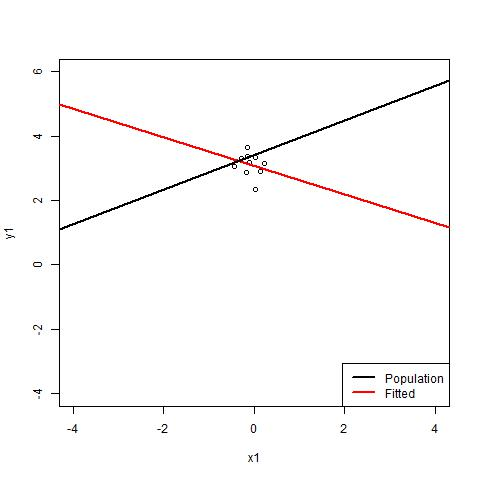
\includegraphics[scale=.5]{vx1.jpg}
%\end{figure}
%\end{center}
%\end{frame}
%\begin{frame}{Var[X]=139}
%\begin{center}
%\begin{figure}
%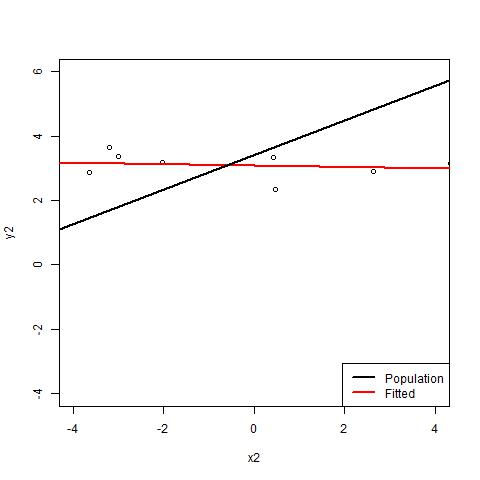
\includegraphics[scale=.5]{vx2.jpg}
%\end{figure}
%\end{center}
%\end{frame}
\begin{frame}{Gauss-Markov 定理}
\begin{theorem}[Gauss-Markov]
OLS假設1到5如果成立,稱為$\textcolor{red}{BLUE} $
\begin{enumerate}
\item Best: 有最小的變異數;
\item Linear: 在所有的線性樣本統計中;
\item Unbiased: 無偏
\item Estimator
\end{enumerate}
\end{theorem}
\end{frame}
\subsection{Error Variance}
\begin{frame}{\H 估計OLS樣本統計的變異數}
\begin{itemize}
\item $\sigma_{u}^2$告訴我們資料的散佈程度。$\sigma_{u}^2$越大,$\hat{\beta}_{0},\hat{\beta}_{1}$對於$\beta_{0},\beta_{1}$的推論也越不佳。
\item 如何估計OLS樣本統計的精確程度?也就是OLS樣本統計的變異數?
\item 利用殘差項
\begin{center} $\hat{u}_{i}=y_{i}-\hat{y}_{i}=y_{i}-\hat{\beta}_{0}-\hat{\beta}_{1}x_{i} $
\end{center}
估計$ Var[u]=\sigma^{2}_{u} $
\item 假設殘差項的分佈可以用
\begin{center}
$ MSD(\hat{u})\equiv\frac{1}{n}\sum\limits_{i=1}^{n}(\hat{u}_{i}-\bar{\hat{u}})^2=\frac{1}{n}\sum\limits_{i=1}^{n}\hat{u}_{i}^2 $
\end{center}
測量。
\item 我們的迴歸線來自於觀察到的資料,$ MSD(\hat{u}) $低估了真實母體迴歸線的誤差量。

\end{itemize}
\end{frame}
\begin{frame}{\H 誤差項變異數的無偏估計}
\begin{itemize}
\item 如果對$ MSD(\hat{u}) $求平均可得到$Var[u] $
\begin{center}
$ E[MSD(\hat{u})]=\frac{n-2}{n}\sigma^{2}_{u} $
\end{center}
\item 因此,誤差項的變異數的無偏估計為:
\begin{align*}
E[MSD(\hat{u})] & =\frac{n-2}{n}\sigma^{2}_{u} \\
\sigma^{2}_{u} & =\frac{n}{n-2}MSD(\hat{u})\\
  & = \frac{n}{n-2}\frac{1}{n}\sum\limits_{i=1}^{n}\hat{u}_{i}^2\\
  & = \frac{1}{n-2}\sum\limits_{i=1}^{n}\hat{u}_{i}^2
\end{align*}
因為估計$\hat{u}_{i}$需要$ \hat{\beta}_{0},\hat{\beta}_{1} $所以自由度為n減2
\end{itemize}
\end{frame}
\begin{frame}
將$ \frac{1}{n-2}\sum\limits_{i=1}^{n}\hat{u}_{i}^2 $代入:\\
$\hat{V}[\hat{\beta}_{1}|X]=\mathlarger{\frac{\sigma_{u}^{2}}{\sum_{i=1}^{n}(x-\bar{x})^2}}=\frac{\sigma_{u}^{2}}{SST_{x}}$\\
$\hat{V}[\hat{\beta}_{0}|X]=\sigma_{u}^{2}\mathlarger{\{\frac{1}{n}+\frac{\bar{x}^2}{\sum_{i=1}^{n}(x-\bar{x})^2}}\}=\mathlarger{\frac{\sigma_{u}^2\sum_{i=1}^{n}x^2}{n\sum_{i=1}^{n}(x-\bar{x})^2}}$\\
$\mathrm{where}$ $\sigma_{u}^{2}=\frac{1}{n-2}\sum\limits_{i=1}^{n}\hat{u}_{i}^2$\\
\medskip
標準誤則是取開根號:$\sqrt{\hat{V}[\hat{\beta}_{0}|X]} $以及$\sqrt{\hat{V}[\hat{\beta}_{1}|X]}$
\end{frame}
\subsection{Normality}
\begin{frame}{\H 誤差項為常態分佈}
\begin{block}{Assumption 6}
根據前面的假設,誤差項與自變項沒有相關,表示為$ u\independent X $。而且假設
\begin{center}
$u\sim N(0,\sigma_{u}^{2})  $
\end{center}
以上假設意義為:
\begin{center}
$  Y|X \sim N(\beta_{0}+\beta_{1}X, \sigma_{u}^{2})$
\end{center}
也就是變異數同質性以及誤差項的平均值為0的假設。
\end{block}
\end{frame}
\begin{frame}{\H 線性迴歸假設}
\begin{itemize}
\item 假設1到6稱為古典線性模型假設($\textcolor{blue}{\textsf {Classical Linear Model assumptions}} $)
\item CLM代表$\textcolor{red}{BUE}$,也就是不論是線性或是非線性的樣本統計,都是變異數最小。
\item 樣本數小的話,呈現常態分佈與否是一個重要的問題。但是變數的轉換可以解決非常態分佈的問題。
\item 而在樣本數夠大的時候,這個假設不一定需要成立。
\end{itemize}
\end{frame}
\begin{frame}{\H \hat{\beta}_{1}}
\begin{theorem}[抽樣分佈]
當假設1到6成立時,
\begin{center}
$\hat{\beta}_{1}\sim N(\beta_{1},Var[\hat{\beta}_{1}|X])$\\
$\mathlarger{Var[\hat{\beta}_{1}|X]=\frac{\sigma_{u}^{2}}{\sum_{i=1}^{n}(x_{i}-\bar{x})^2} } $
\end{center}
換句話說,
\begin{center}
$\mathlarger{\frac{\hat{\beta}_{1}-\beta_{1}}{\sqrt{Var[\hat{\beta}_{1}|X]}}=\frac{\hat{\beta}_{1}-\beta_{1}}{\sqrt{Var[\hat{\beta}_{1}|X]}}=\frac{\hat{\beta}_{1}-\beta_{1}}{SE(\hat{\beta})}\sim N(0,1)}$
\end{center}
\end{theorem}
這是因為:
\begin{center}
$ \hat{\beta}_{1} = \beta_{1}+\sum\limits_{i=1}^{n}\frac{(x-\bar{x})^2}{SST_{x}} u_{i}$\\
$u_{i}\sim N(0,\sigma_{u}^{2})$
\end{center}
常態分佈的變數的線性組合是線性,而且常態分佈可標準化為$ N(0,1) $
\end{frame}

\begin{frame}\frametitle{\H 總結}
\begin{enumerate}
\item {\K 瞭解何謂線性假設}
\item {\K 瞭解何謂隨機抽樣}
\item {\K 瞭解何謂X有變異量}
\item {\K 瞭解何謂誤差項的平均值為0}
\item {\K 瞭解何謂變異同質性}
\item {\K 瞭解何謂誤差項成常態分佈}
\item {\K 瞭解哪些假設必須成立}
\end{enumerate}
\end{frame}

\end{document}
